\documentclass[../main.tex]{subfiles}
\graphicspath{{\subfix{../images/}}}

\begin{document}

\section{Materials and Methods}

\subsection{Equipment}
This research has been conducted on a first-generation \davinci surgical system decommissioned in 2016 and equipped with the dVRK (\davinci Research Kit) framework. The dVRK \cite{Kazanzides2014} is an open-source mechatronics system, consisting of electronics, firmware, and software, that is being used to control research systems based on the first-generation \davinci systems. Based on a ROS \cite{Quigley2009} framework, the dVRK implements high-level accessibility to the sensors, actuators and control algorithms of the \davinci robot, making it more easily interfaceable with advanced strategies and algorithms developed in the most diverse software environments.

The simulator developed for this project renders necessary only the surgeon console, as the ROS messages are sent solely to the virtual surgical scene and not to the physical robot. However, all features of the \psms and of the \ecm are implemented: the \hrsv shows the 3D virtual surgical scene, the \mtms correctly controls the virtual surgical tools, and the clutch foot-switch allows proper repositioning maneuvers. 

\subsection{The Surgical Simulator} 
The objective of investigating a high-specificity aspect regarding the impact of \vfs introduced the necessity of developing an \textit{ad-hoc} surgical simulator with specialized surgical tasks and training exercises: this would allow quantifying surgical performance and monitor training over the key surgical skills as indicated by Smith \textit{et al.} in \cite{Smith2014}. 

The simulator is based on \textit{Unity}, a cross-platform game engine that allows the development of 3D applications and games. The Unity engine is a powerful tool for the development of virtual environments, as it allows the creation of complex 3D scenes with a high level of realism, and the implementation of complex interactions between the virtual objects and the user. Specifically, the simulator implements gravity, object collisions and manipulation. A 3D model of the \davinci patient cart is present in the simulator and responds in real-time to the ROS messages received from the console, therefore the virtual \psms replicate the motion of the real ones. 

Two virtual cameras are positioned in the Unity scene on the tip of the endoscope mounted on the \ecm: the horizontal distance between the two virtual cameras ($5.3 \unit{mm}$) matches the one of the real endoscope, as does the Field-of-View ($80 \unit{deg^2}$). The feeds of the virtual cameras, rendering the 3D scene in real-time, are sent separately to the two oculars of the \hrsv. The slightly different images from the left and right eye yield the sensation of depth perception and allow the user to perceive the virtual scene in three dimensions, as it happens when teleoperating with the real robot. 

The training surgeon interacts with the console in the same exact way as he would when teleoperating in the \ac{or}: he views the surgical scene in the oculars, the virtual instruments respond in real-time to the movements of the manipulators and with the same kinematics, and the 3D objects behave in the same way as they would if they were real thanks to the simulated physics computed by the Unity Engine.   

\subsubsection{The Surgical Tasks}
The simulator comprises eight surgical tasks, four of which (\textit{Path, Rings, Pillars} and \textit{Exchange}) are simplistic training tasks built with objects of simple geometry, while the remaining four (\textit{Liver Resection, Nephrectomy, Thymectomy} and \textit{Suturing}) emulate \textit{in-vivo} surgical procedures and are therefore more realistic. Fig.\ref{fig:taskspanel} collects snapshots of the tasks. All of these are constructed and set up in order to be as challenging as possible in relation to a specific surgical skill. Specifically:

\begin{itemize}
  \item \textit{Path} and \textit{Liver Resection} require articulate wrist motion and stability
  \item \textit{Rings} and \textit{Nephrectomy} survey the depth perception skills
  \item \textit{Pillars} and \textit{Thymectomy} are hand-eye coordination tasks
  \item \textit{Exchange} and \textit{Suturing}, both bi-manual tasks, challenge the capabilities in terms of instrument exchange 
\end{itemize}

\begin{figure}
    \centering
    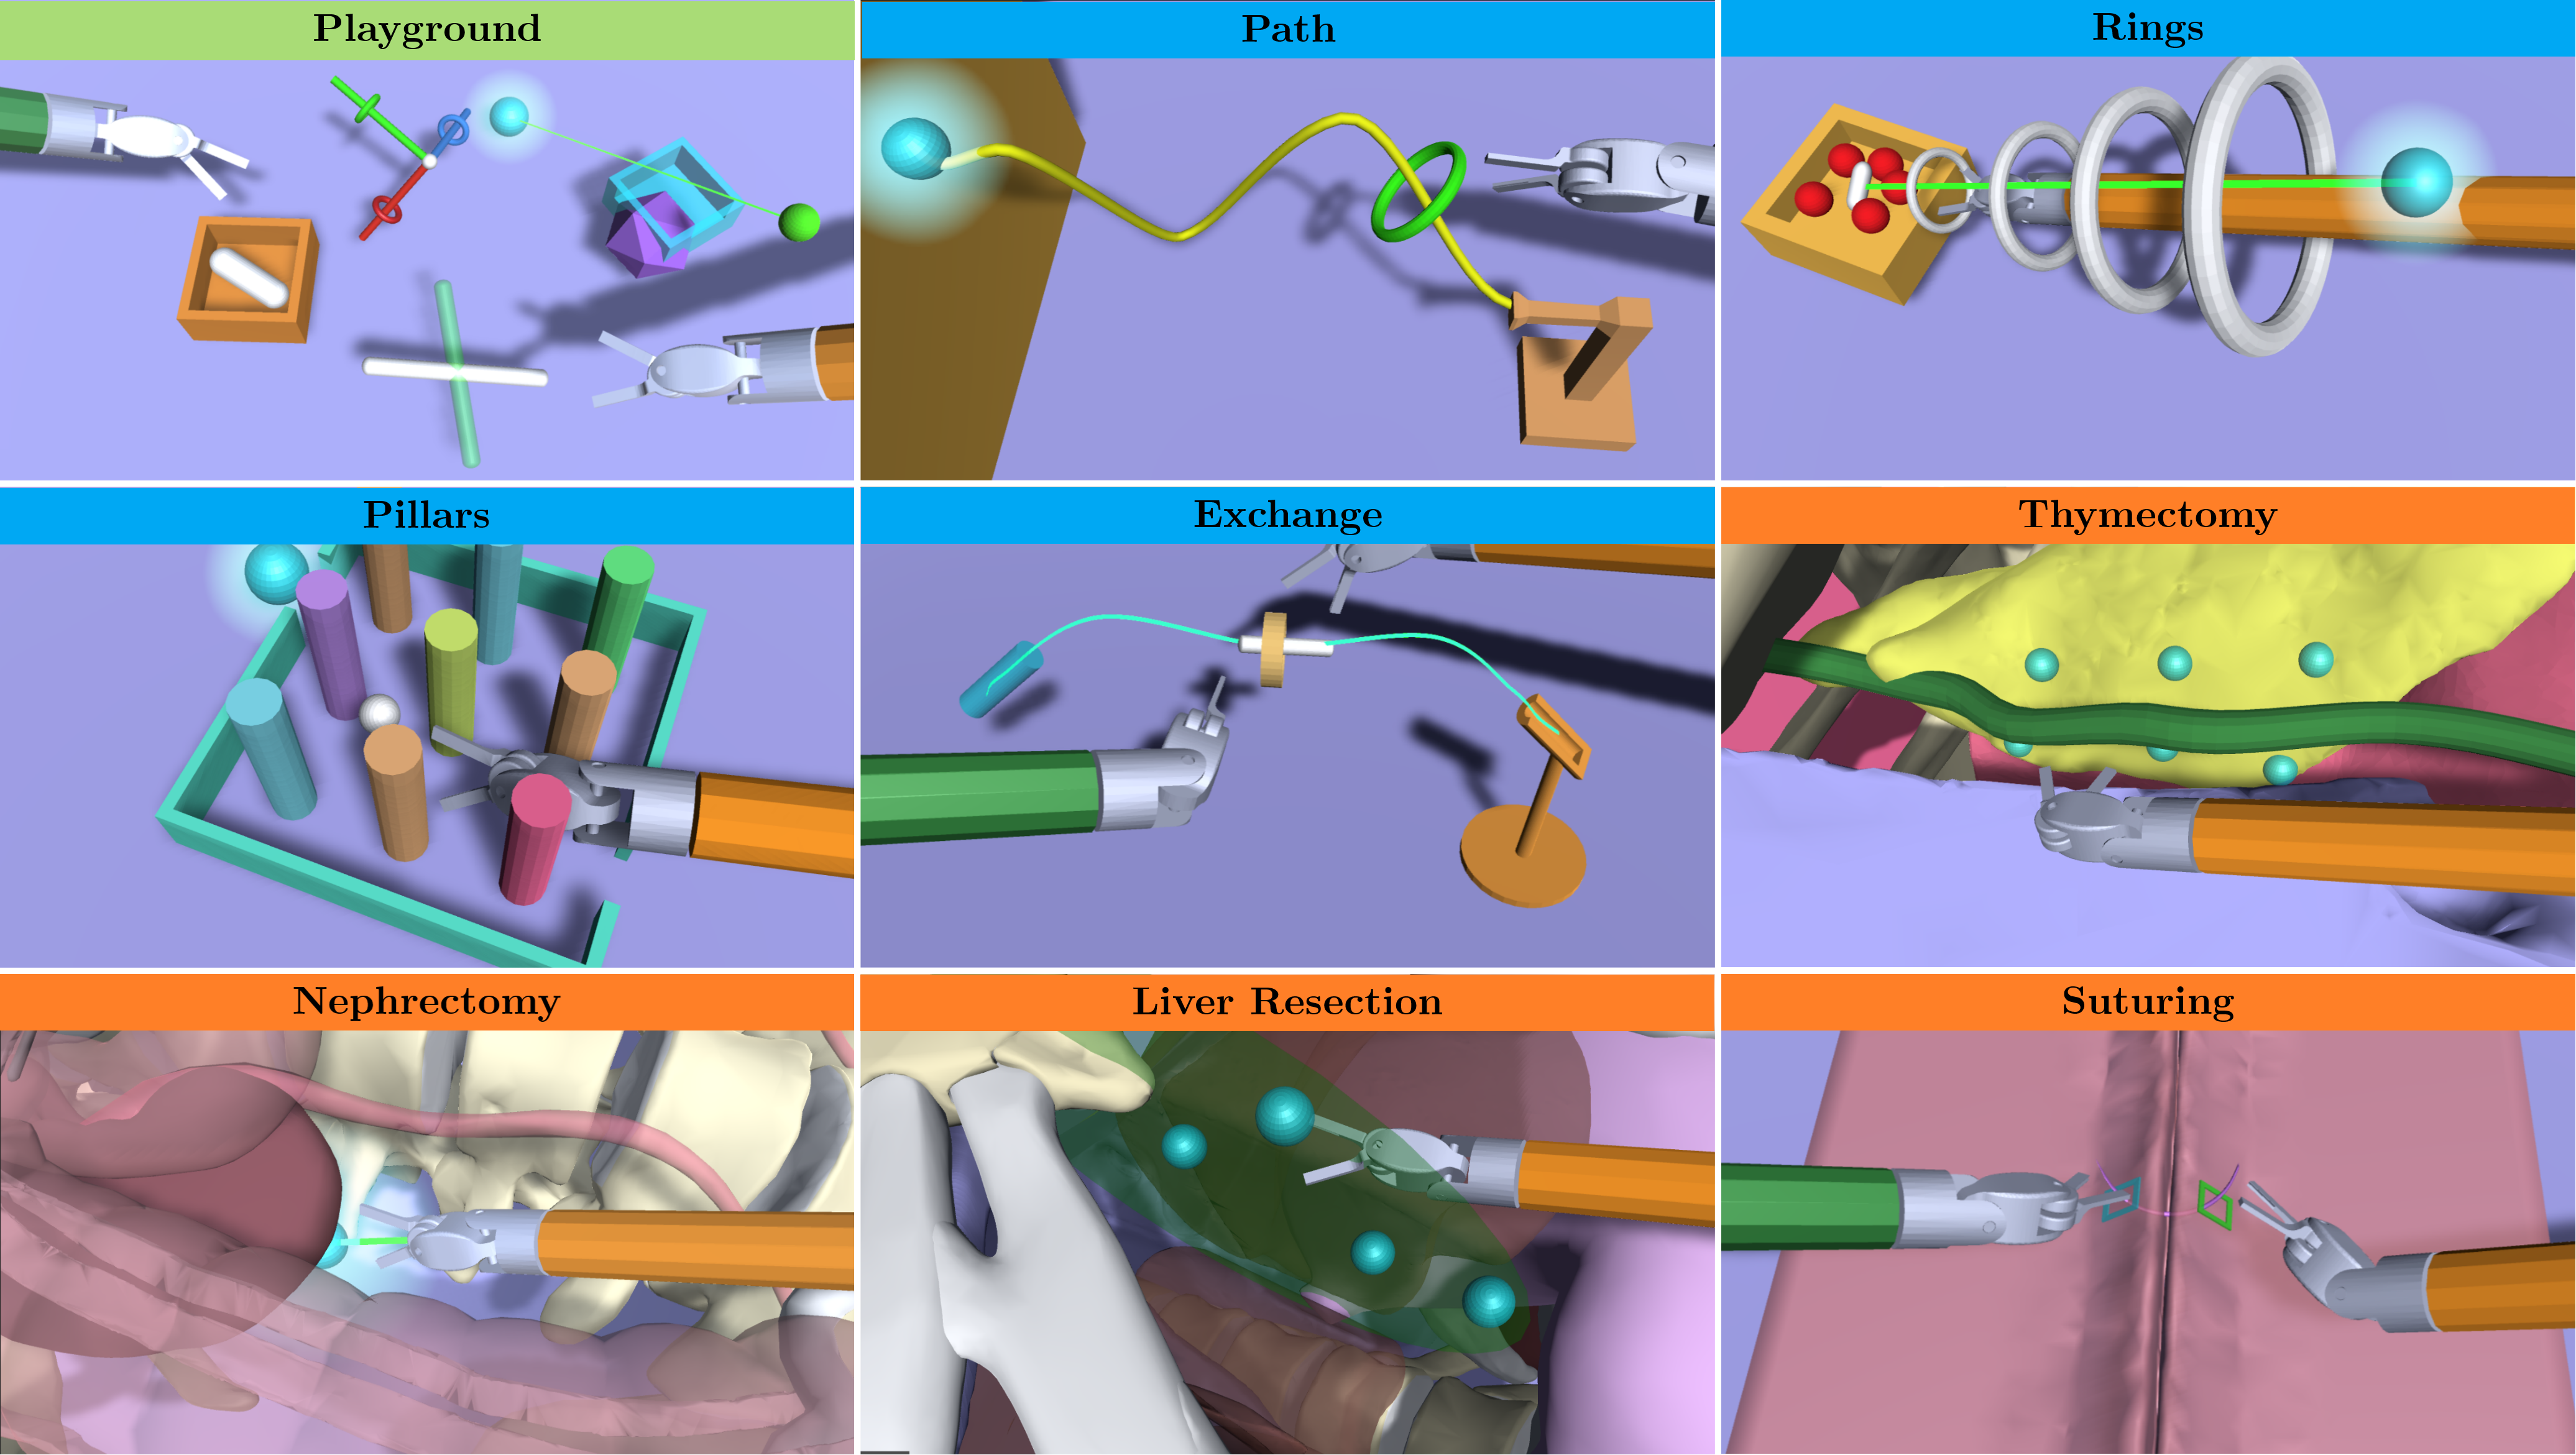
\includegraphics[width=\textwidth]{images/tasks_panel.png}
    \caption{Snapshot of the simulated surgical tasks, with the respective denomination. Training tasks have blue headlines, while realistic evaluation tasks have orange headlines. \textit{Playground} is a propaedeutic task and isn't featured in the experimental study}
    \label{fig:taskspanel}
\end{figure}

\paragraph{Path} Objective of this task is to grab a torus-like object and carry it along a reference trajectory. To achieve this, discrete wrist articulation and motion smoothness are required. The reference trajectory is set up in order to require a wrist rotation of at least $90 \unit{deg}$ around 2 perpendicular axes, the one pointing from right to left and the one pointing forward with respect to the camera view.
\paragraph{Rings} In this task, the operator is required to precisely insert the instrument inside a narrow constrained space defined by a set of increasingly smaller rings, grab a target object and carry it out of the constrained space. The task tests the depth perception skills of the operator, as the rings are positioned at an angle with respect to the camera view.
\paragraph{Pillars} This task test the trainee's steady-hand skills, as well as hand-eye coordination. While carrying an object through a set of obstacles that most times obscure the free path, the operator is also required to extrapolate the path that he must take to reach the intended target.
\paragraph{Exchange} To test the bi-manual coordination and the ability to exchange an object from one hand to another, this task demands the operator to carry a cylinder-shaped object from a starting position to a target location, exchanging it from the right to the left hand at the mid-point of the path. 
\paragraph{Thymectomy} In a surgical thymectomy, a lobe of the thymus gland is cut and removed. The vicinity of the so delicate phrenic nerve requires the utmost care and precision and, in most cases, a minimally-invasive approach is, indeed, preferred. In the emulated version of this task, the surgeon shall pinch a set of 6 targets located on the surface of the virtual thymus while staying as far as possible from the phrenic nerve. 
\paragraph{Nephrectomy} A careful insertion of the surgical instrument inside the abdominal cavity is required to perform a nephrectomy. The insertion is often performed at a steep angle with respect to the camera view, and the surgeon must be able to perceive the depth of the target object. This virtual nephrectomy re-creates both of these aspects.
\paragraph{Liver Resection} The surgeon must perform a series of cuts along the surface between two lobes of the liver to perform a successful liver resection. Naturally, to minimize tissue damage, the instrument's tooltip shall remain as close as possible to the surface between the two lobes to be separated.
\paragraph{Suturing} Suturing with a recurve circular needle is a challenging task requiring the medical doctor to approach the tissue at an optimal angle and to properly exchange the needle from one hand to the other.  
\paragraph{Playground} This propaedeutic task allows the trainee to familiarize himself with the simulator and the virtual surgical tools. A few simple objects are scattered Win the scene and the trainee is free to interact with them. The scope of this task is to better interface a novice user with teleoperation and the \ac{vr} environment, understanding how its movements are mapped to the motion of the instruments, how to perform a pinching action and what intensity of force and torque to expect when \vfs are applied. 


\subsection{Virtual Fixtures}
The tasks as described in the previous paragraph are equipped, in the virtual environment, with high-level assistance strategies that act applying mechanical forces to the \mtms, with the aim of re-directing the motion of the surgeon's arm towards intended targets or away from obstacles. The \mtms are, indeed, 8-DOFs robotic actuated arms (the last degree of freedom is not actuated and controls the opening and closing of the gripper with a magnetic Hall sensor): each of the 7 rotational joints is equipped with both an encoder for sensing purposes and with a motor for actuation purposes. The encoders determine the joint angles that will ultimately be used for estimating the pose of the gripper in the console's space, through FK; it's this pose, transformed with respect to the \hrsv \rf, that the \psms are actuated to recreate, with respect to the endoscope \rf, as in Fig.\ref{fig:consoletocarttransform}. 

\begin{figure}[h]
    \centering
    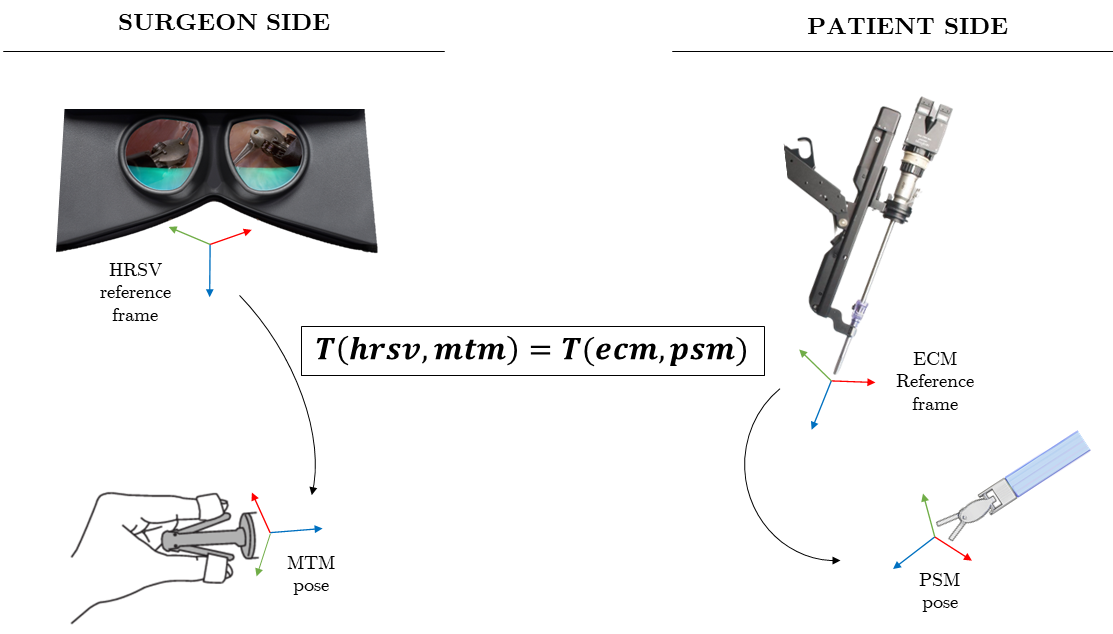
\includegraphics[width=\textwidth]{images/console_to_cart_transform.png}
    \caption{The equivalence of transformations between the console space and the surgical space. The transformation matrix that expresses the pose of the manipulator in the \hrsv reference frame is used to compute the desired pose of the \psm in the \rf of the endoscope camera.}
    \label{fig:consoletocarttransform}
\end{figure}

In the real surgical context, the motors are used to automatically position the manipulators at the start of the procedure, for gravity compensation and for exploiting the redundancy of the kinematic chain to optimally position the links of the \mtm in order to avoid collisions with the surgeon's wrist. However, the same dynamic model used for these purposes can be exploited to apply assistive mechanical forces to the manipulators, the direction and magnitude of which are determined from the pose of the \psms's tooltip in the surgical \rf. A force to be applied to the manipulator tooltip is converted to the set of torques to be applied at each joint by the respective actuators. The parameters of this inverse dynamics model \cite{Fontanelli2017} for the generic i-\textit{th} link are:
\begin{itemize}
  \item The mass $m_i$ of the link
  \item The three components of the first moment $\textbf{m}_i$ of the link
  \item The six independent elements of the inertia tensor $\textbf{I}_i$ of the link
  \item The static and viscous coefficients of the link, $F_{s,i}$ and $F_{v,i}$ respectively
\end{itemize}

The \vf force computed in the virtual surgical space - in the simulator - is therefore converted, in real-time, to a set of 7 torques to be communicated as a ROS message to the \mtms. 
The same inverse dynamics model converts a torque to be applied to the end effector into a set of 7 torques to be applied to the joint motors. 

\subsubsection{Error Mapping}
Most of the assistance strategies implemented here will use the distance from the \psm to the target or obstacle as the primary metric for determining the intensity of the feedback force or torque. However, different surgical tasks and situations require a level of control over how the distance is taken into account. For this reason a sigmoidal mapping function is employed for the normalization of the linear or angular error into a suitable interval. Specifically, such mapping is formulated as:

\begin{equation}
  f_{map}(x) = \frac{1}{1+e^{5\delta w(x-t-h)}}
  \label{eq:sigmoidalmap}
\end{equation}

with $\delta = +1$ for guidance \vfs and $\delta = -1$ for avoidance \vfs ($\delta$ determines if the function increases or decreases monotonically). Here:
\begin{itemize}
  \item $t$ is the fixture \textit{threshold}, hence the value at which the sigmoid starts to significantly increase from zero
  \item $h$ is the distance from the threshold at which \textit{half} of the maximum force is provided
  \item $w$ controls the \textit{width} of the linear region, hence the steepness of the curve 
\end{itemize}
For example, if $t=2\si{mm}$ and $h=3\si{mm}$ the surgeon will start to feel a force for errors higher than 2\si{mm}, and at 5\si{mm} he will experience half of the maximum force that can be delivered.

\begin{figure}[h!]
  \centering
      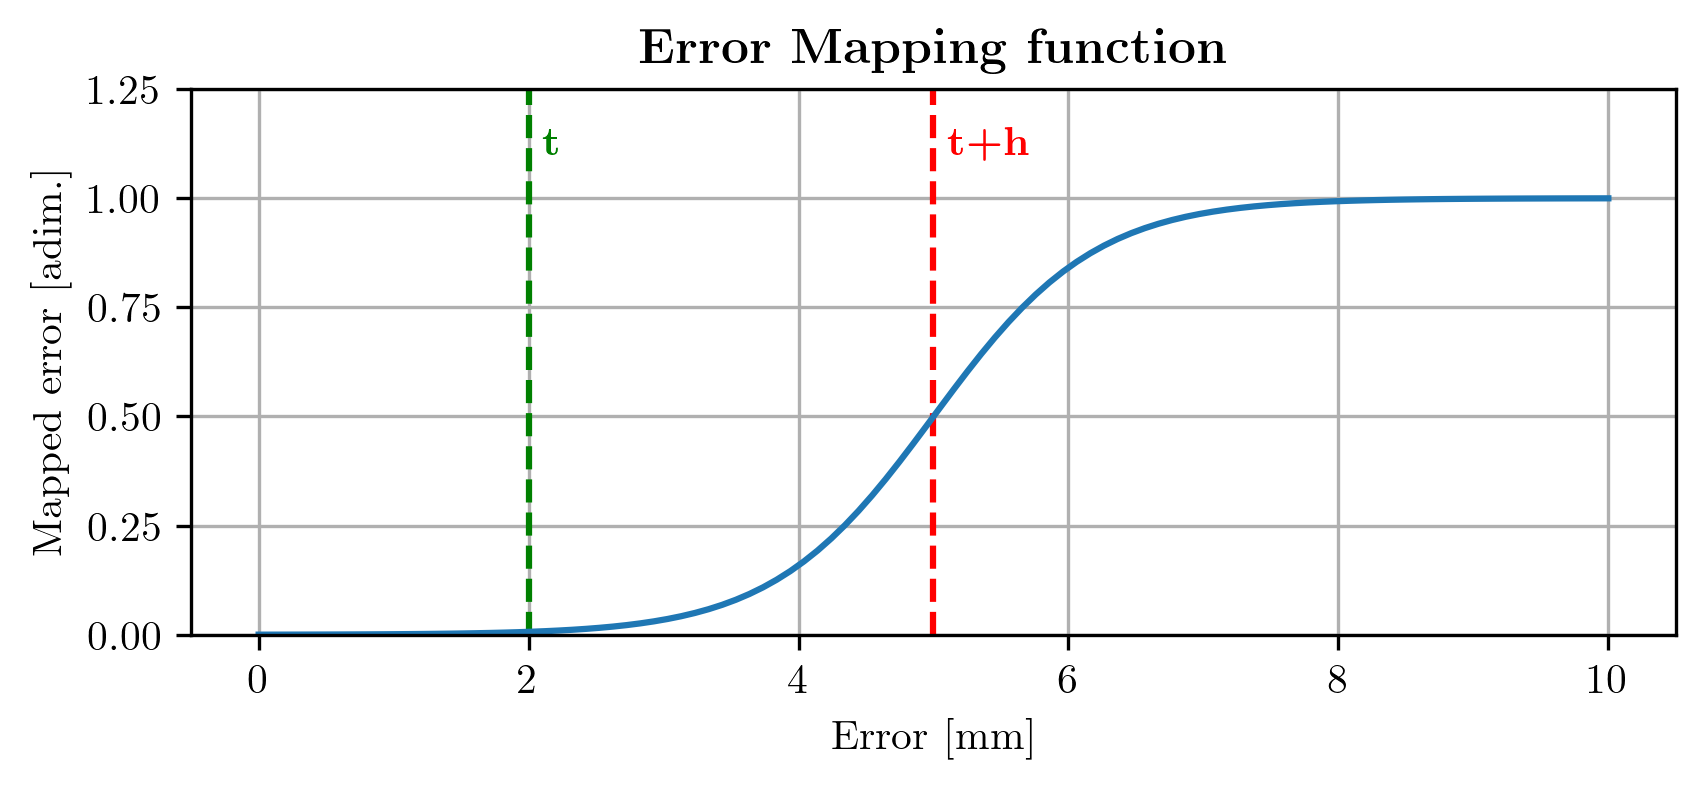
\includegraphics[width=0.75\textwidth]{images/mappingfunction.png}
      \caption{Plot of the Error Mapping function. The position of$t$ and $t+h$ can be set manually to achieve a suitable behavior of the assistance strategy. The x-axis refers to a generic error shown in millimeters, but the same mapping function can be applied to an angular error.} 
      \label{fig:mappingfunctiion}
\end{figure}

$t$, $h$ and $w$ are set manually in order to achieve an optimal "feeling" of the \vf. Their values, different from task to task, are reported in Tab.\ref{tab:thwvalues}.

\begin{table}
    \centering
    \caption{Error mapping parameters for the different tasks. \textit{Exchange}, \textit{Liver Resection} and \textit{Suturing} map both the distance error and the angular error, so the values of both mapping functions are reported.}
    \begin{tabular}{||c||c|c|c||}
        \hline
        \textbf{Task} & $\textbf{t} $ & $\textbf{h}$ & $\textbf{w}$ \\
        \hline\hline
        Path            & 2 mm & 2 mm & 500 \\ 
        \hline
        Rings           & 2 mm & 2 mm & 500 \\ 
        \hline
        Pillars         & 0.5 mm & 1 mm & 1000 \\ 
        \hline
        Exchange (distance)        & 3 mm & 2 mm & 500 \\ 
        \hline
        Exchange (angular)        & 5$^{\circ}$  & 5$^{\circ}$ & 2 \\ 
        \hline
        Thymectomy      & 0.5 mm & 1 mm & 1000 \\ 
        \hline
        Nephrectomy     & 2 mm & 2 mm & 500 \\ 
        \hline
        Liver Resection (distance) & 2 mm & 5 mm & 200 \\ 
        \hline
        Liver Resection (angular) & 5$^{\circ}$ & 15$^{\circ}$ & 1\\ 
        \hline
        Suturing (distance) & 1 mm & 3 mm & 300 \\ 
        \hline
        Suturing (angular) & 5$^{\circ}$ & 5$^{\circ}$ & 2\\ 
        \hline
    \end{tabular}
    \label{tab:thwvalues}
\end{table}

\subsubsection{Virtual Fixtures Algorithms}
As stated previously the force feedback delivered at the level of \mtm is computed, in terms of magnitude and direction, from the surgical space and therefore based on the relative position and orientation of the \psm's tooltip with respect to the objects in the virtual surgical scene. The simulator features 4 assistance algorithms implementing 4 different declinations of haptic assistance. Different algorithms are deployed inside specific surgical tasks based on the task morphology and goals:
\begin{itemize}
  \item \textbf{Trajectory Guidance:} This algorithm outputs a force vector that assists the surgeon in following a pre-defined 3D trajectory. A visco-elastic force pulls the \ee tooltip towards the closest point of the trajectory, and a visco-elastic toorque aligns the tooltip's orientation with the trajectory tangent vector, computed at the closest point.
  \item \textbf{Obstacle Avoidance:} An Obstacle Avoidance algorithm prevents the practicioner from colliding with the virtual objects in the scene, which may represent, for example, delicate anatomical structures that must not be touched during surgery. A visco-elastic force is, therefore, applied to the \ee tooltip in order to push it away from the closest point of the obstacle.
  \item \textbf{Insertion Guidance:} Some surgical tasks require the insertion of the instrument's tooltip into a narrow space. This algorithm, from an initial position of the \psm and a target position, aid the surgeon in approaching the target on an optimal insertion path, without deviating from it.
  \item \textbf{Surface Guidance:} After defining, in the pre-operative stage, an ideal surface of operation (the surface can be of any morphology and should be defined as a mesh of points), a Surface Guidance algorithm generates forces and torques that keep the surgical tool on such surface and with an orientation tangent to it. 
\end{itemize} 

Fig.\ref{fig:vfsgraphics} graphically illustrates the \vf algorithms as described above, but a detailed analytical formulation of each algorithm follows in the next sections.

\begin{figure}
    \centering
    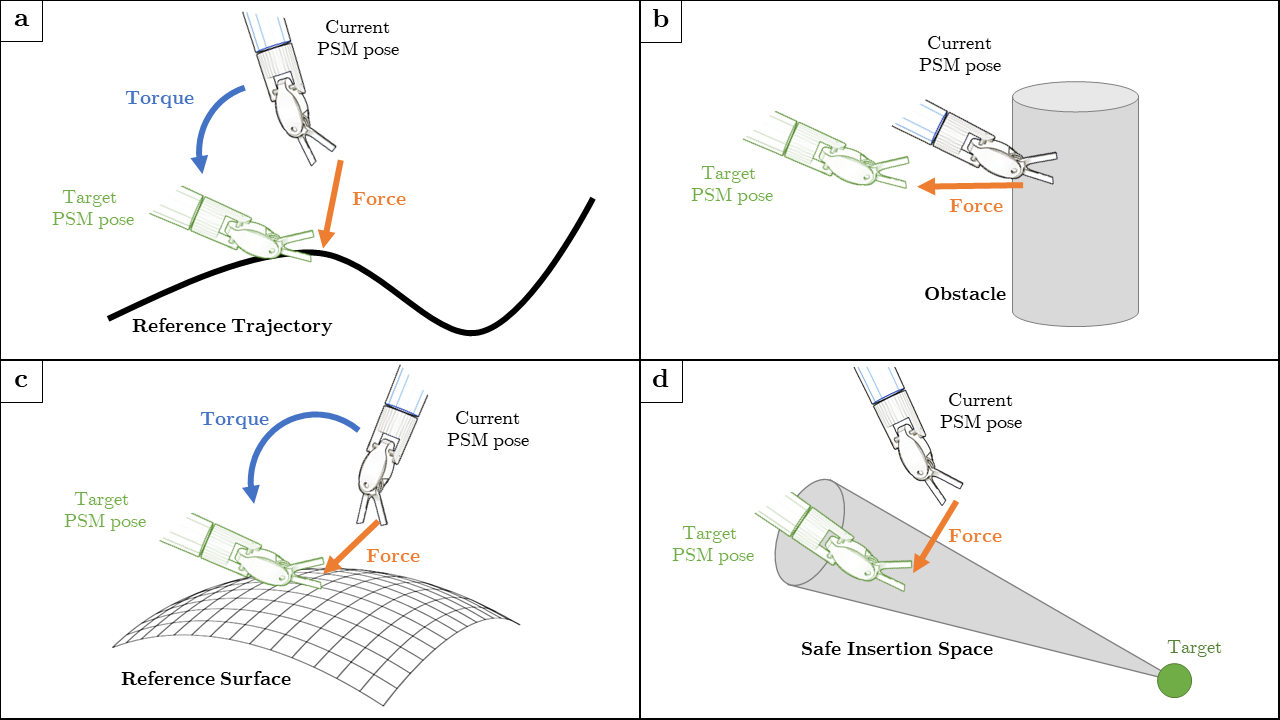
\includegraphics[width=\textwidth]{images/vfs_graphics.png}
    \caption{Graphics scheme of the 4 virtual fixtures featured as assistance strategies in the surgical simulator. \textbf{a.} Trajectory Guidance; \textbf{b.} Obstacle Avoidance; \textbf{c.} Surface Guidance; \textbf{d.} Insertion Guidance. A representative \psm's pose is shown, and a target pose is also depicted in a green hue, together with the force (orange arrows) and torque (blue arrows) that will guide the motion toward the target pose.}
    \label{fig:vfsgraphics}
\end{figure}

\paragraph{Trajectory Guidance} 
Considering a generic three-dimensional trajectory planned in the pre-operative stage, the feedback forces will be calculated according to the relative position and orientation of the trajectory itself and the tooltip reference frame. Both the forces and torques are computed in real-time as the sum of an elastic and a viscous contribution: while the elastic component accounts for the positional or angular error to the closest point of the reference trajectory - and the tangent computed in such point, accordingly - the viscous components are proportional to the temporal rate of change of the errors themselves. 

A viscoelastic model allows to achieve a guidance and error-compensating assistance that is less prone to overshooting behaviors and to oscillations. Moreover, with the force and torque being calculated as 
\begin{equation}
    \vect{F} = k_F\cdot\vect{F}_{elastic} + \eta_F\cdot\vect{F}_{viscous} 
    \label{eq:force}
\end{equation}
\begin{equation}
    \vect{T} = k_T\cdot\vect{T}_{elastic} + \eta_T\cdot\vect{T}_{viscous}
    \label{eq:torque}
\end{equation}
one tunes the elastic gains $k_F$ and $k_T$ and the viscous damping coefficients $\eta_F$ and $\eta_T$ in order to achieve a comfortable balance between the components and a stable behavior of the feedback force, which may vary from operator to operator, as well as from task to task.

Fig. \ref{fig:vfsgraphics}a illustrates the vectors involved in the computation of the virtual fixture; specifically, contributions in Eq.\ref{eq:force} expanded as:
\begin{equation}
    \vect{F}_{elastic} = \vect{d}
\end{equation} 
\begin{equation}
    \vect{F}_{viscous} = 
    \begin{cases} 
        \vect{d}, & \textit{if         } \vect{v}\cdot\vect{d}<0 \\
         rotate(\vect{v},\theta,\vect{r}), & \textit{otherwise}
    \end{cases}
\end{equation} 

Here, $\vect{d}$ is the distance vector going from the surgical instrument to the closest point in the trajectory, $\vect{v}$ is the velocity of the surgical instrument, while $\theta$ and $\vect{r}$ are the angle and axis of rotation which will align the velocity vector $\vect{v}$ with $\vect{d}$, respectively:
\begin{equation}
    \theta = (1+\vect{v}\cdot\vect{d})\cdot\frac{\pi}{2}
\end{equation}
\begin{equation}
    \vect{r} = \vect{v}\times\vect{d}
\end{equation}
This implementation is adapted from \cite{Enayati2016}. Similarly, contributions to the torque (Eq.\ref{eq:torque}) are expanded as: 
\begin{equation}
    \vect{T}_{elastic} = acos (\vect{z}\cdot\vect{t} ) \cdot \vect{z} \times \vect{t}
    \label{eq:telastic}
\end{equation}
\begin{equation}
    \vect{T}_{viscous} = \frac{d}{dt} \left[ acos (\vect{z}\cdot\vect{t} ) \right] \cdot \vect{z} \times \vect{t}
    \label{eq:tviscous}
\end{equation}
The role of the torque is to align the z-axis of the surgical tool's reference frame with the tangent of the trajectory $\vect{t}$ at its closest point. In Eq.\ref{eq:telastic} and Eq.\ref{eq:tviscous}, the angle and axis of rotation which will achieve this alignment are $acos(\vect{z}\cdot\vect{t})$ and $\vect{z} \times \vect{t}$, respectively.

\paragraph{Obstacle Avoidance}
\paragraph{Surface Guidance}
\paragraph{Insertion Guidance}


\subsection{Clinical Validation}
\subsection{Experimental Protocol}
\subsection{Performance Metrics}


% BIBLIOGRAPHY
\bibliographystyle{unsrt}
\bibliography{refs.bib}

\end{document}